% =============================================================================
%  REPORTE DE PRÁCTICA — Materia de Verano: Internet of Things
%  Universidad Panamericana · Ingeniería Mecatrónica · 6.° semestre
%
%  INSTRUCCIONES PARA EL ALUMNO:
%    1. Abre este archivo en overleaf.com (gratis, no requiere instalación)
%    2. Rellena TODOS los campos marcados con  %%  ESCRIBE AQUÍ
%    3. Inserta tus capturas de pantalla donde indica el comentario
%    4. Compila con el botón verde de Overleaf antes de entregar
%    5. Entrega el PDF generado + sube el .tex a tu repositorio de GitHub
% =============================================================================

\documentclass[12pt, letterpaper]{article}

% ── Paquetes ──────────────────────────────────────────────────────────────────
\usepackage[utf8]{inputenc}
\usepackage[spanish]{babel}
\usepackage[T1]{fontenc}
\usepackage{geometry}
\usepackage{graphicx}
\usepackage{float}
\usepackage{amsmath}
\usepackage{booktabs}
\usepackage{array}
\usepackage{xcolor}
\usepackage{listings}
\usepackage{hyperref}
\usepackage{fancyhdr}
\usepackage{titlesec}
\usepackage{caption}
\usepackage{enumitem}
\usepackage{parskip}
\usepackage{mdframed}
\usepackage{multirow}
\usepackage{tabularx}
\usepackage{linegoal}
\usepackage{amssymb}

% ── Márgenes ──────────────────────────────────────────────────────────────────
\geometry{top=2.5cm, bottom=2.5cm, left=2.5cm, right=2.5cm}

% ── Colores ───────────────────────────────────────────────────────────────────
\definecolor{upBlue}     {HTML}{2E3A59}
\definecolor{roseMain}   {HTML}{C2547A}
\definecolor{roseLight}  {HTML}{FAE8EF}
\definecolor{tealMain}   {HTML}{0F6E56}
\definecolor{tealLight}  {HTML}{E1F5EE}
\definecolor{amberMain}  {HTML}{854F0B}
\definecolor{amberLight} {HTML}{FAEEDA}
\definecolor{grayLight}  {HTML}{F5F5F5}
\definecolor{grayMid}    {HTML}{AAAAAA}
\definecolor{codeBack}   {HTML}{F5F5F5}
\definecolor{codeComment}{HTML}{6A7F6A}
\definecolor{codeKeyword}{HTML}{7B4DB0}
\definecolor{codeString} {HTML}{B85C00}

% ── Estilo de código ─────────────────────────────────────────────────────────
\lstdefinestyle{arduino}{
  language        = C++,
  backgroundcolor = \color{codeBack},
  basicstyle      = \ttfamily\small,
  keywordstyle    = \color{codeKeyword}\bfseries,
  commentstyle    = \color{codeComment}\itshape,
  stringstyle     = \color{codeString},
  numberstyle     = \tiny\color{gray},
  numbers         = left,
  numbersep       = 8pt,
  stepnumber      = 1,
  frame           = single,
  framerule       = 0.5pt,
  rulecolor       = \color{roseMain},
  breaklines      = true,
  captionpos      = b,
  tabsize         = 2,
  showstringspaces= false,
  literate        = {á}{{\'a}}1 {é}{{\'e}}1 {í}{{\'i}}1
                    {ó}{{\'o}}1 {ú}{{\'u}}1 {ñ}{{\~n}}1
                    {Á}{{\'A}}1 {É}{{\'E}}1 {Í}{{\'I}}1
                    {Ó}{{\'O}}1 {Ú}{{\'U}}1 {Ñ}{{\~N}}1
}
\lstset{style=arduino}

% ── Estilo de secciones ───────────────────────────────────────────────────────
\titleformat{\section}
  {\large\bfseries\color{upBlue}}{\thesection.}{0.5em}{}
  [\color{roseMain}\titlerule]

\titleformat{\subsection}
  {\normalsize\bfseries\color{upBlue}}{\thesubsection.}{0.5em}{}

\titleformat{\subsubsection}
  {\normalsize\bfseries\color{roseMain}}{\thesubsubsection.}{0.5em}{}

% ── Encabezado y pie ─────────────────────────────────────────────────────────
\pagestyle{fancy}
\fancyhf{}
\fancyhead[L]{\small\color{upBlue} Reporte de Práctica — IoT}
\fancyhead[R]{\small\color{upBlue} Universidad Panamericana}
\fancyfoot[C]{\small\color{gray}\thepage}
\renewcommand{\headrulewidth}{0.4pt}
\renewcommand{\footrulewidth}{0.4pt}
\renewcommand{\headrule}{%
  \hbox to\headwidth{\color{roseMain}\leaders\hrule height\headrulewidth\hfill}}

% ── Caja de instrucción (para el alumno) ─────────────────────────────────────
\newenvironment{instruccion}{%
  \begin{mdframed}[
    backgroundcolor = tealLight,
    linecolor       = tealMain,
    linewidth       = 1pt,
    innerleftmargin = 10pt, innerrightmargin = 10pt,
    innertopmargin  = 6pt,  innerbottommargin= 6pt
  ]
  \small\color{tealMain}\textbf{Instrucción:}\hspace{4pt}\color{black}
}{%
  \end{mdframed}
}

% ── Caja de nota / advertencia ───────────────────────────────────────────────
\newenvironment{notaBox}[1][Nota]{%
  \begin{mdframed}[
    backgroundcolor = amberLight,
    linecolor       = amberMain,
    linewidth       = 1pt,
    innerleftmargin = 10pt, innerrightmargin = 10pt,
    innertopmargin  = 6pt,  innerbottommargin= 6pt
  ]
  \small\textbf{\color{amberMain}#1:}\hspace{4pt}
}{%
  \end{mdframed}
}

% ── Espacio para respuesta (líneas en blanco) ─────────────────────────────────
% Uso: \respuesta{5}  →  deja 5 líneas en blanco con líneas guía
\newcommand{\respuesta}[1]{%
  \vspace{4pt}%
  \foreach \i in {1,...,#1}{%
    \noindent\textcolor{grayMid}{\rule{\linewidth}{0.3pt}}\\[10pt]%
  }%
}

% ── Celda de tabla en blanco con fondo gris claro ───────────────────────────
\newcommand{\celda}{\cellcolor{grayLight}}

% ── Hipervínculos ─────────────────────────────────────────────────────────────
\hypersetup{colorlinks=true, linkcolor=upBlue, urlcolor=roseMain}

% ── Paquete necesario para \foreach ──────────────────────────────────────────
\usepackage{pgffor}
\usepackage{colortbl}


% =============================================================================
\begin{document}
% =============================================================================

% ── Portada ───────────────────────────────────────────────────────────────────
\begin{titlepage}
  \centering

  {\color{upBlue}\rule{\linewidth}{1.5pt}}\\[0.4cm]

  {\Large \textbf{\color{upBlue} Universidad Panamericana}}\\[0.2cm]
  {\large Facultad de Ingeniería}\\[0.2cm]
  {\large Ingeniería Mecatrónica · 6.° semestre}\\[0.4cm]

  {\color{roseMain}\rule{\linewidth}{0.8pt}}\\[1cm]

  {\LARGE \textbf{\color{upBlue} Reporte de Práctica}}\\[0.5cm]

  % ── Número y nombre de la práctica ────────────────────────────────────────
  {\huge \textbf{\color{roseMain}
    Práctica 1} :%% NÚMERO DE PRÁCTICA
    \vspace{0.3cm}\\
    \underline{\hspace{9cm}}          %% NOMBRE DE LA PRÁCTICA
  }\\[0.8cm]

  {\large \textbf{Materia de Verano: Internet of Things (IoT)}}\\[2cm]

  % ── Datos del equipo ──────────────────────────────────────────────────────
  \begin{tabular}{rl}
    \textbf{Alumno 1:}  & Marco Alberto Vázquez Preciado \\[0.5em]%% TU NOMBRE
    \textbf{Alumno 2:}  & Jaime Valencia Rodríguez \\[0.5em]%% NOMBRE COMPAÑERO
    \textbf{Profesor:}  & Zyanya Alejandra Orozco Olivares \\[0.5em] %% NOMBRE PROFESOR
    \textbf{Semana:}    & 1era Semana\\[0.5em] %% SEMANA Y DÍA
    \textbf{Fecha:}     & \today                              \\[0.5em]
    \textbf{GitHub:}    & https://github.com/0263136-JVR/Practicas-IoT \\[0.5em] %% URL DE TU REPO
  \end{tabular}\\[2cm]

  {\color{upBlue}\rule{\linewidth}{1.5pt}}
  \vfill
  {\small\color{gray} Materia de Verano · Universidad Panamericana · \the\year}
\end{titlepage}

% ── Tabla de contenido ────────────────────────────────────────────────────────
\tableofcontents
\newpage


% =============================================================================
\section{Objetivo}
% =============================================================================

\begin{instruccion}
  Describe en 2 o 3 oraciones el propósito de la práctica. Explica
  \textbf{qué querías lograr}, no el procedimiento. Usa tus propias palabras.
\end{instruccion}

El objetivo de esta practica es lograr utilizar la funcionalidad de Bluetooth Low Energy (BLE) disponible en nuestra ESP32, y con ello, lograr una conexion entre un celular y la placa para poder enviar informacion desde un dispositivo hacia el otro, y viceversa.


% =============================================================================
\section{Marco teórico}
% =============================================================================

\begin{instruccion}
  Explica los conceptos clave que aplicaste. Escribe con tus propias palabras —
  no copies definiciones. Mínimo 3 subsecciones. Agrega las que necesites.
\end{instruccion}

% ── 2.1 ──────────────────────────────────────────────────────────────────────
\subsection{Bluetooth Low Energy (BLE)}

\emph{Bluetooth Low Energy}, mejor conocido como BLE, es un protocolo de envio de informacion enfocado en enviar pocos datos, a una corta distancia, conservando la mayor cantidad de energia posible. Esta protocolo permite que un dispositivo cliente logre enviar, leer y recibir notificaciones de un dispositivo servidor.

Cuenta con tres propiedades clave: \emph{Read, Write y Notify}. La primera le permite leer los datos disponibles cuando quiera, es decir, puede tomar datos que se le enviaron siempre y cuando se utilize esta funcion. La segunda es write, la cual permite escribir datos y enviarlos hacia el otro dispositivo. La ultima funcion, al igual que write, envia informacion hacia el otro dispositivo, pero, para recibir esta, no es necesario leerla, sino que simplemente se recibe en el dispositivo.

Gracias a su eficiencia, rapida conexion y amplia compatibilidad, BLE es ampliamente utilizado en monitoreo, automatizacion e Internet de las Cosas (IoT).

% ── 2.2 ──────────────────────────────────────────────────────────────────────
\subsection{Arquitectura GATT}

\begin{instruccion}
  Explica la jerarquía GATT (perfil, servicio, característica, descriptor)
  y qué significa cada nivel. Puedes usar la siguiente tabla como apoyo.
\end{instruccion}

\begin{table}[H]
  \centering
  \caption{Jerarquía GATT — completa la columna de explicación}
  \begin{tabular}{>{\bfseries\color{roseMain}}p{3cm}
                  >{\centering\arraybackslash}p{3.5cm}
                  p{5.5cm}}
    \toprule
    \textbf{\color{upBlue}Elemento} &
    \textbf{\color{upBlue}Ejemplo del proyecto} &
    \textbf{\color{upBlue}¿Qué es? (con tus palabras)} \\
    \midrule
    Perfil GATT    & El ESP32 del motor   & Es el encargado de todo el software y de la conexion BLE, es decir, es el cerebro de nuestro proyecto.\\[1.5em]
    Servicio       & Servicio Motor       & Todo lo relacionado al control y monitoreo del motor. \\[1.5em]
    Característica & RPM, Setpoint, Temp. & Es una variable dentro del sistema la cual puede ser modificada por una de sus propiedades.\\[1.5em]
    Propiedad      & Read, Write, Notify  & Las propiedades del protocolo BLE. Le permite leer, enviar y forzar datos hacia otro dispositivo.\\[1.5em]
    Descriptor     & CCCD (BLE2902)       & Permite que el cliente habilite o deshabilite las notificaciones y las indicaciones.\\[1.5em]
    \bottomrule
  \end{tabular}
\end{table}

% ── 2.3 ──────────────────────────────────────────────────────────────────────
\subsection{Roles BLE: Central y Peripheral}

\textbf{Central:} Es el dispositivo que busca, inicia y administra la conexion BLE. Ademas de esto, el Central puede leer, escribir y recibir las caracteristicas del dispositivo Peripheral. Un ejemplo de estos es un celular, o una computadora.

\textbf{Peripheral:} Es el dispositivo que anuncia sus servicios BLE y espera a que un dispositivo Central se conecte. Ya que el dispositivo Central se conecta, envia sus caracteristicas a este mismo para que las pueda utilizar. En esta practica, nuestra ESP32 funciona como dispositivo Peripheral, esperando la conexion del celular hacia el.


% =============================================================================
\section{Materiales y equipo}
% =============================================================================

\begin{instruccion}
  Enlista todos los componentes que utilizaste. Agrega filas si es necesario.
\end{instruccion}

\begin{table}[H]
  \centering
  \caption{Materiales utilizados}
  \begin{tabular}{clcc}
    \toprule
    \textbf{\#} & \textbf{Componente} & \textbf{Cantidad} & \textbf{Observaciones} \\
    \midrule
    1 & Computadora& 1& Arduino IDE instalado\\[0.4em]
    2 & ESP32& 1& Funcion de BLE requerida\\[0.4em]
 3& Celular& 1&Aplicacion nRF instalada\\
  \end{tabular}
\end{table}


% =============================================================================
\section{Diagrama de conexiones}
% =============================================================================

\begin{instruccion}
  Inserta una foto o diagrama de tus conexiones físicas. Si la práctica no
  requirió conexiones externas al ESP32, descríbelo brevemente en texto.
  Para insertar una imagen: guarda el archivo como \texttt{diagrama.png}
  en la misma carpeta que este \texttt{.tex} y descomenta las líneas de abajo.
\end{instruccion}

% Descomenta y ajusta cuando tengas tu imagen:
% \begin{figure}[H]
%   \centering
%   \includegraphics[width=0.75\textwidth]{diagrama.png}
%   \caption{Diagrama de conexiones}
%   \label{fig:diagrama}
% \end{figure}

Para esta practica, no se requirieron conexiones externas a la placa. La unica conexion usada durante la practica fue por medio del puerto USB de la computadora, hacia el puerto USB-C de la ESP32. Esta conexion se utilizo tanto para energizar la placa, como para programarla.


% =============================================================================
\section{Desarrollo y procedimiento}
% =============================================================================

\subsection{Configuración del entorno de desarrollo}

\begin{instruccion}
  Describe los pasos que seguiste para configurar PlatformIO y el proyecto.
  Incluye tu archivo \texttt{platformio.ini} real (el que usaste tú, con tus
  librerías) en el siguiente bloque de código.
\end{instruccion}

\begin{lstlisting}[caption={platformio.ini — tu configuración real}, label={lst:platformio}]
#include <BLEDevice.h>
#include <BLEServer.h>
#include <BLEUtils.h>
#include <BLE2902.h>

#define SERVICE_UUID "b989f340-9c88-4c80-8d1e-88105b8ef1d9"
#define CHAR_RPM_UUID "9b149b6d-205a-4813-b40c-e1703422620a"
#define CHAR_SETPOINT_UUID "6b857f1b-3b69-404b-a7c7-e1e4992fd157"

//variables globales
BLEServer* pServer = nullptr;
BLECharacteristic* pRpmChar = nullptr;

bool deviceConnected = 0;

float rpm = 0.0;
float setpoint = 0.0;

class ServerCallbacks : public BLEServerCallbacks{

  void onConnect (BLEServer* s){
    deviceConnected = true;

    Serial.println(">>> Central concectado!");
  }

  void onDisconnect(BLEServer* s){
    deviceConnected = false;
    s->startAdvertising();

    Serial.println(">>> Central desconcectado!");
  }
};

class SetPointCallbacks : public BLECharacteristicCallbacks{

  void onWrite(BLECharacteristic* c){
    String val = c->getValue();

    if(val.length() > 0){
      setpoint = atof(val.c_str());

      Serial.printf("Setpoint: %.1f RPM\n",setpoint);
    }
  }

};
\end{lstlisting}

\subsection{Implementación del código}

\begin{instruccion}
  Pega tu código fuente completo (\texttt{main.cpp}) en el bloque de abajo.
  Asegúrate de que sea la versión que subiste a GitHub — con tus UUIDs reales.
\end{instruccion}

\begin{lstlisting}[caption={main.cpp — código fuente de la práctica}, label={lst:main}]
void setup() {
  Serial.begin(115200);

  //Step 1: BLE INIT
  BLEDevice::init("Motor_JVMA");

  //Step 2: Server & Callbacks
  pServer = BLEDevice::createServer();
  pServer->setCallbacks(new ServerCallbacks());

  //Step 3: Service
  BLEService* pService = pServer->createService(SERVICE_UUID);

  //Set 4: Notify
  pRpmChar = pService->createCharacteristic(
    CHAR_RPM_UUID,
    BLECharacteristic::PROPERTY_READ | BLECharacteristic::PROPERTY_NOTIFY
  );
  pRpmChar->addDescriptor(new BLE2902);

  //Step 5: Write
  BLECharacteristic* pSpChar = pService->createCharacteristic(
    CHAR_SETPOINT_UUID,
    BLECharacteristic::PROPERTY_WRITE
  );
  pSpChar->setCallbacks(new SetPointCallbacks());

  //Step 6: Service & advertising
  pService->start();

  BLEAdvertising* pAdv = BLEDevice::getAdvertising();
  pAdv->addServiceUUID(SERVICE_UUID);

  pAdv->setScanResponse(true);

  BLEDevice::startAdvertising();

  Serial.println("BLE listo - esperando conexion...");
}

void loop() {
  if(deviceConnected){
    //Simulate enconder lectura
    rpm +=5;

    if(rpm > 600.0) rpm = 0.0;

    //Convert float->String & Notify
    char buf[10];
    sprintf(buf, "%.1f", rpm);
    pRpmChar->setValue(buf);
    pRpmChar->notify();

    //Log serial monitor
    Serial.printf("RPM: %.1f | Setpoint: %.1f\n", rpm, setpoint);
  }

  delay(500);
}
\end{lstlisting}

\subsection{Procedimiento de prueba}

\begin{instruccion}
  Describe paso a paso lo que hiciste para probar que el sistema funcionaba.
  Sé específico: menciona qué herramientas usaste, qué observaste en cada paso
  y cómo verificaste que el resultado era correcto.
\end{instruccion}

\begin{enumerate}[leftmargin=1.5cm]
  \item Copiamos el codigo que nos proporciono la maestra para la practica. Este estaba conformado por algunas clases, el setup y el loop.
  \item Definimos nuestras UUIDs para el servidor, las RPMs y el setpoint, ademas del nombre del dispositivo.
  \item Compilamos y revisamos todos los errores de sintaxis que teniamos.
  \item Corregimos los errores y ejecutamos el codigo.
  \item Dentro de la nRF en el celular, buscamos el dispositivo bluetooth y nos conectamos a el.
  \item Revizamos el monitor serial para comprobar que los datos se estuvieran enviando.
  %% Agrega más pasos si los necesitas
\end{enumerate}


% =============================================================================
\section{Resultados}
% =============================================================================

\subsection{Capturas de pantalla}

\begin{instruccion}
  Inserta al menos 2 capturas de pantalla: una del Serial Monitor y una
  de la app nRF Connect mostrando los datos recibidos. Guárdalas como
  \texttt{serial.png} y \texttt{nrf.png} en la misma carpeta que el \texttt{.tex}.
\end{instruccion}

% Captura 1: Serial Monitor
 \begin{figure}[H]
   \centering
   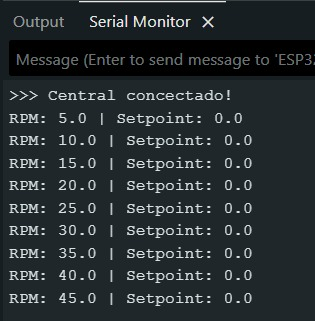
\includegraphics[width=0.85\textwidth]{serial.png}
   \caption{Salida del Serial Monitor durante la práctica}
   \label{fig:serial}
 \end{figure}

% Captura 2: nRF Connect
 \begin{figure}[H]
   \centering
   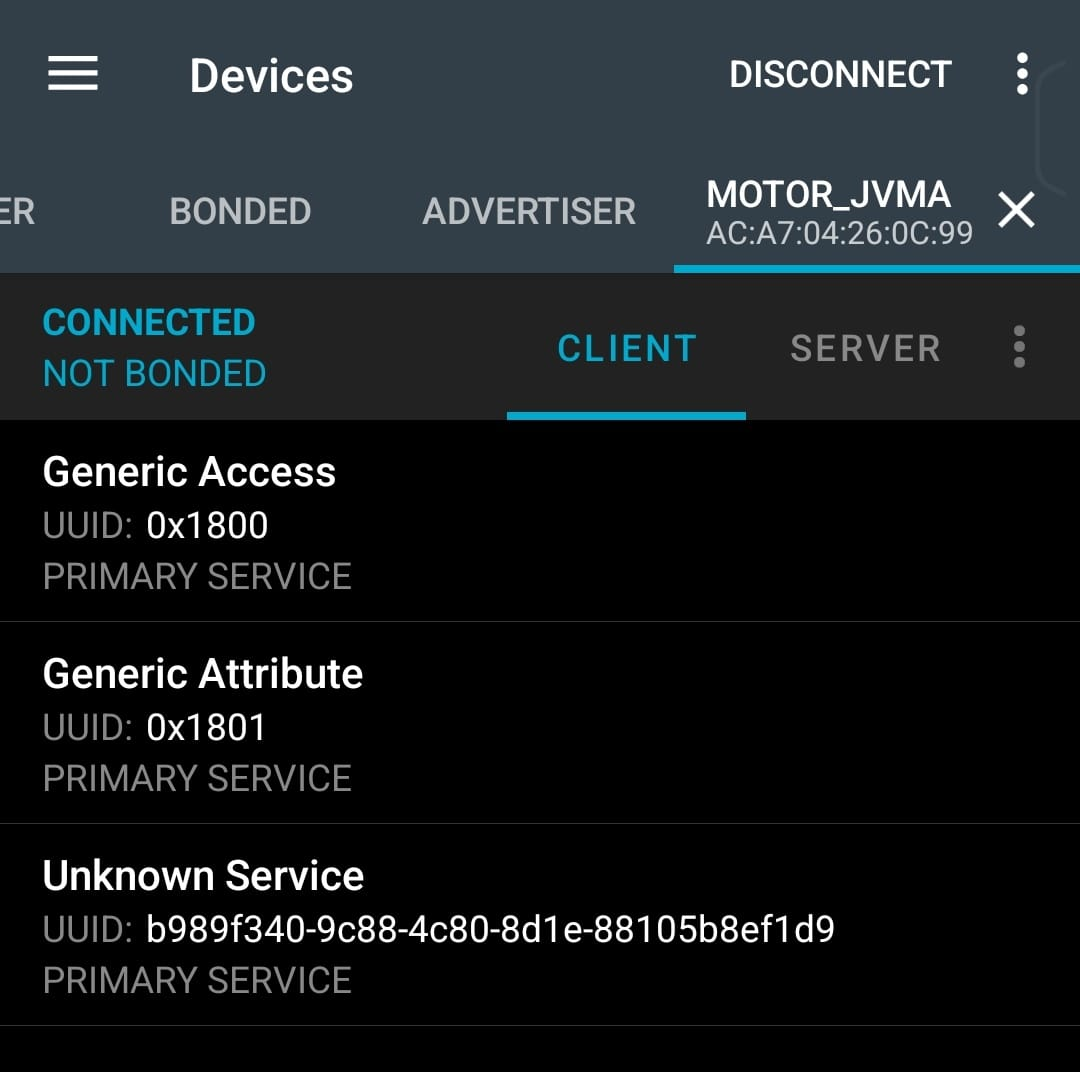
\includegraphics[width=0.5\textwidth]{nrf.png}
   \caption{App nRF Connect mostrando los valores recibidos}
   \label{fig:nrf}
 \end{figure}



\subsection{Tabla de resultados}

\begin{instruccion}
  Llena la tabla con los valores que observaste durante la práctica.
  Los valores de la columna derecha deben ser datos reales — no los esperados.
\end{instruccion}

\begin{table}[H]
  \centering
  \caption{Resultados observados durante la prueba}
  \begin{tabular}{lcc}
    \toprule
    \textbf{Variable medida / observada} &
    \textbf{Valor esperado} &
    \textbf{Valor observado} \\
    \midrule
    Frecuencia de Notify (actualizaciones/s) & 2 Hz       & NA\hspace{4cm} \\[0.6em]
    Rango de RPM simuladas                   & 0–600 RPM  & 0-600 RPM \\[0.6em]
    Setpoint enviado desde nRF Connect       & 500.0 RPM  & 500.0 RPM \\[0.6em]
    Setpoint recibido (Serial Monitor)       & 500.0 RPM  & 0.0 RPM \\[0.6em]
    RSSI medido (dBm)                        & Negativo   & -65 dBm \\[0.6em]
    Tiempo de conexión BLE (s)               & $<$ 3 s    & NA \\[0.6em]
    %% Agrega más filas si midiste otras variables
    \bottomrule
  \end{tabular}
\end{table}

\subsection{Registro del Serial Monitor}

\begin{instruccion}
  Copia y pega un fragmento representativo de la salida real de tu Serial
  Monitor. Debe incluir: el mensaje de inicio, al menos una conexión, varios
  ciclos de RPM y la recepción de un setpoint.
\end{instruccion}

\begin{lstlisting}[language={}, caption={Fragmento real del Serial Monitor}]
BLE listo - esperando conexion...
>>> Central concectado!
RPM: 5.0 | Setpoint: 0.0
RPM: 10.0 | Setpoint: 0.0
RPM: 15.0 | Setpoint: 0.0
RPM: 20.0 | Setpoint: 0.0
RPM: 25.0 | Setpoint: 0.0
RPM: 30.0 | Setpoint: 0.0
>>> Central desconcectado!
\end{lstlisting}


% =============================================================================
\section{Análisis y discusión}
% =============================================================================

\begin{instruccion}
  No repitas los resultados. Interprétalos: explica el \textbf{por qué}
  de lo que observaste. Mínimo 3 subsecciones.
\end{instruccion}

% ── 7.1 ──────────────────────────────────────────────────────────────────────
\subsection{¿Por qué es necesario el descriptor \texttt{BLE2902}?}

Porque es aquel que nos permite que la comunicación sea de forma eficiente sin desperdiciar energía extra en procesamientos al ser el encargado de habilitar o no la posibilidad de notificación entre el cliente y el servidor.
 
% ── 7.2 ──────────────────────────────────────────────────────────────────────
\subsection{¿Qué ocurriría si se omite \texttt{startAdvertising()} en \texttt{onDisconnect}?}

Lo que ocurriría sería que la ESP o el servidor se volvería totalmente invisible al momento de desconectarse por primera vez, lo que causaría que fuera imposible una reconexión con el mismo u otro cliente, a menos de que se reinicie el programa, algo que necesita intervención física y para nada es la idea de un IoT.

% ── 7.3 ──────────────────────────────────────────────────────────────────────
\subsection{Diferencia entre las propiedades READ, WRITE y NOTIFY}

\begin{table}[H]
  \centering
  \caption{Comparativa de propiedades GATT — completa con tus propias palabras}
  \begin{tabular}{>{\bfseries}p{2cm} p{4.5cm} p{4.5cm}}
    \toprule
    \textbf{Propiedad} &
    \textbf{¿Quién inicia la transferencia?} &
    \textbf{¿Cuándo usarla en este proyecto?} \\
    \midrule
    READ    & El cliente & Cuando es necesario consultar el estado actual del motor, o el inicial al conectarse por primera vez \\[2.5em]
    WRITE   & El cliente & Para enviar configuraciones o nuevos valores de control hacia el motor. Nuevo valor de Setpoint \\[2.5em]
    NOTIFY  & El servidor & Para datos en tiempo real que cambian constantemente y a alta velocidad, como el valor de RPM \\[2.5em]
    \bottomrule
  \end{tabular}
\end{table}

% =============================================================================
\section{Respuestas a preguntas de análisis}
% =============================================================================

\begin{instruccion}
  Responde cada pregunta con al menos 3 oraciones. Fundamenta tus respuestas
  con lo que observaste en el laboratorio.
\end{instruccion}

\begin{enumerate}[leftmargin=1.5cm, label=\textbf{P\arabic*.}]

  % ── Pregunta 1 ───────────────────────────────────────────────────────────
  \item \textbf{¿Cuáles son los tres canales de advertising en BLE y por qué
        están ubicados estratégicamente dentro de la banda de 2.4 GHz?}

Para una ESP son los canales 37, 38 y 39, y están distribuidos de esta forma para evitar interferencia por parte del Wi-Fi, haciendo que no estén una misma zona juntos sino repartidos en los espacios libres que deja el otro protocolo.
\\

  % ── Pregunta 2 ───────────────────────────────────────────────────────────
  \item \textbf{¿Por qué se usa \texttt{atof(val.c\_str())} para procesar
        el valor recibido en el callback \texttt{onWrite}? ¿Qué tipo de dato
        devuelve y por qué es necesaria la conversión?}

Se usa para que cuando se envie datos desde el cliente en forma de escritura, que están en formato de texto ASCII se pueda convertir en un valor de tipo flotante y pueda ser interpretado por el código como un número.
\\

  % ── Pregunta 3 ───────────────────────────────────────────────────────────
  \item \textbf{¿Cuál es la diferencia entre un UUID estándar del Bluetooth SIG
        (como \texttt{0x180F}) y un UUID personalizado de 128 bits? ¿Cuándo
        conviene usar cada uno?}

La diferencia entre estos UUID es que el estándar es más corto, de 16 bits, y ya están definidos para ciertos servicios de sensores o dispositivos disponibles en el mercado; a diferencia de los personalizados que son más largos pero nos permiten configurar dispositivos nuevos que no necesariamente esten estandarizados.
\\
  % ── Pregunta 4 ───────────────────────────────────────────────────────────
  \item \textbf{¿En qué parte del código se controla la frecuencia de
        actualización de las notificaciones de RPM? ¿Qué implicaciones tiene
        reducir ese valor a 100 ms o aumentarlo a 2000 ms?}

Dicha frecuencia de actualización se controla al final del bloque loop a través del delay, y el estar modificandolo haría que la velocidad de actualización sea más rápida, con riesgo de pérdida de paquetes por saturación, o lenta con gran eficiencia energética pero sin una noción de tiempo real sobre los datos.
\\

  % ── Pregunta 5 ───────────────────────────────────────────────────────────
  \item \textbf{¿Cómo podrías modificar el código para que el ESP32 deje de
        enviar notificaciones automáticamente y solo responda cuando el Central
        las solicita explícitamente? ¿Qué propiedad usarías?}

Se tendría que dejar de enviar los datos de forma automática y hacerlo únicamente bajo petición del cliente cambiando la caracterísitca de RPM de NOTIFY a READ. Esto a través de modificar el or de la caracterísitica creada para el RPM eliminando propiedad de notificación, y eliminando su descriptor de tipo BLE2902 ya que la información no deberá ser mandada recurrentemente en forma de " suscripción"
\\

\end{enumerate}


% =============================================================================
\section{Conclusiones}
% =============================================================================

\begin{instruccion}
  Escribe \textbf{mínimo 3 conclusiones numeradas}. Cada conclusión debe:
  (a) ser específica y verificable con los resultados de esta práctica,
  (b) no ser una opinión general, y
  (c) poder respaldarse con un dato real de tu tabla de resultados o captura.
\end{instruccion}

\begin{enumerate}[leftmargin=1.5cm]
  \item A través de esta práctica se logró inicializar de forma correcta el protocolo de comunicación BLE a través de la programación de una ESP32 como se nota en las capturas de prueba.
  \item Se evidenció la necesidad de un reinicio de evento a través del método startAdvertising() ante una desconexión ya que de no ser así rompe la permanencia inalámbrica del servidor eliminando la posibilidad de una reconexión.
  \item Aún desconocemos el mandado de datos a partir del cliente, en su caracterísitca WRITE, pese a comprender su inicialización en el servidor no se ha intentado realizar dicho segmento en el código, hecho que será necesario para el desarrollo del proyecto.
  %% Agrega una cuarta si tienes algo relevante que decir
\end{enumerate}


% =============================================================================
\section{Repositorio y entregables}
% =============================================================================

\begin{instruccion}
  Completa la información de tu repositorio. Verifica que el enlace funcione
  antes de entregar — el profesor revisará que el código en GitHub sea el mismo
  que pegaste en la sección 5.2.
\end{instruccion}

\vspace{0.5cm}

\begin{tabular}{rl}
  \textbf{URL:}&
    https://github.com/0263136-JVR/Practicas-IoT/blob/main/Practica1/\\[0.6em]%% PEGA TU URL AQUÍ
  \textbf{Rama:} &
    main\\[0.6em]%% ej. main / semana1
  \textbf{Carpeta:}&
    Practica1\\[0.6em]%% ej. semana1/dia2_ble/
  \textbf{Último commit:}&
    08 / 07 / 2026\\[0.6em] %% antes de la demo del viernes
\end{tabular}

\vspace{0.8cm}

\begin{notaBox}[Lista de verificación antes de entregar]
  Marca cada ítem cuando esté completo:
  \begin{itemize}[leftmargin=1.5cm, label=$\square$]
    \item PDF compilado sin errores en Overleaf
    \item Portada con datos correctos (nombres, fecha, GitHub)
    \item Código real pegado en las secciones 5.1 y 5.2
    \item Capturas de pantalla insertadas (Serial Monitor + nRF Connect)
    \item Tabla de resultados con valores reales observados
    \item Las 5 preguntas de análisis respondidas
    \item Mínimo 3 conclusiones
    \item Repositorio de GitHub actualizado con el código de la práctica
    \item Archivo \texttt{.tex} subido al repositorio de GitHub
  \end{itemize}
\end{notaBox}


% =============================================================================
\section*{Referencias}
% =============================================================================

\begin{instruccion}
  Enlista \textbf{todas} las fuentes que consultaste. Mínimo 3.
  Formato: Autor. \textit{Título}. Año. URL o editorial.
\end{instruccion}

\begin{thebibliography}{9}

  \bibitem{ref1}
   \textbf{Android Developers. \textit{Bluetooth de bajo consumo (Bluetooth Low Energy)}.} 2025. \href{https://developer.android.com/develop/connectivity/bluetooth/ble/ble-overview?hl=es-419}{https://developer.android.com/develop/connectivity/bluetooth/ble/ble-overview?hl=es-419} 

  \bibitem{ref2}
    \textbf{Novel Bits. \textit{Bluetooth Low Energy (BLE): The Beginner's Guide}.} 2023. \href{https://novelbits.io/bluetooth-low-energy-ble-complete-guide/}{https://novelbits.io/bluetooth-low-energy-ble-complete-guide/} 

  \bibitem{ref3}
    \textbf{Bluetooth Special Interest Group (Bluetooth SIG). \textit{The Bluetooth® Low Energy Primer}.} 2022. \href{https://www.bluetooth.com/bluetooth-resources/the-bluetooth-low-energy-primer/}{https://www.bluetooth.com/bluetooth-resources/the-bluetooth-low-energy-primer/} 

  %% Agrega más referencias si las usaste

\end{thebibliography}


\end{document}